\documentclass[11pt]{article}

\usepackage[utf8]{inputenc}
\usepackage{fancyhdr}
\usepackage{hyperref}
\usepackage{graphicx}

\graphicspath{ {images/} }
 
\pagestyle{fancy}
\fancyhf{}
\lhead{University of the Witwatersrand}
\rfoot{School of Computer Science and Applied Mathematics}
\pagenumbering{roman}
\fancyfoot[R]{\thepage}

\begin{document}
\begin{page}

\newcommand{\HRule}{\rule{\linewidth}{0.3mm}} % Defines a new command for the horizontal lines, change thickness here
\renewcommand\section{\@startsection{section}{1}{\z@}%
                                  {-3.5ex \@plus -1ex \@minus -.2ex}%
                                  {2.3ex \@plus.2ex}%
                                  {\normalfont\large\bfseries}}
\setlength{\parindent}{0pt}

\center % Center everything on the page
 
%----------------------------------------------------------------------------------------
%	HEADING SECTIONS
%----------------------------------------------------------------------------------------

\textsc{\LARGE University of the Witwatersrand}\\[1.5cm] % Name of your university/college
\textsc{\Large School of Computer Science and Applied Mathematics}\\[0.5cm] % Major heading such as course name

%----------------------------------------------------------------------------------------
%	TITLE SECTION
%----------------------------------------------------------------------------------------

\HRule \\[0.4cm]
{ \huge \bfseries COMS3008: Parallel Computing Lab Assignment 2}\\[0.4cm] % Title of your document \\
  \large 25 July 2016
\HRule \\[1.5cm]
 
%----------------------------------------------------------------------------------------
%	AUTHOR SECTION
%----------------------------------------------------------------------------------------
\begin{minipage}{1\textwidth}
	\Large \emph By Chalom, J. (711985)\\
\end{minipage}


\vfill % Fill the rest of the page with whitespace

\end{page}

\begin{page}

\clearpage
\setcounter{page}{1}
\pagenumbering{arabic}

\section{General Assumptions}
The system for which the decomposition of the factorial algorithm is to be used has only two processing units. Each unit is identical with their own exclusive memory and also have shared memory spaces between them. The factorial algorithm being investigated will have 1 as the last number multiplied to the running variable in order to find the factorial os some integer $n$.

\section{Directed Acyclic Graphs}
\noindent \chapter{Chosen Decomposition:} \\
\noindent Let $n$ be the number whose factorial is being investigated. \\
$ n = \{ n \in \mathbb{Z}\ |\ 1 \leq n \leq \mathbb{Z}\} $ 
\\

\begin{figure}
\centering
     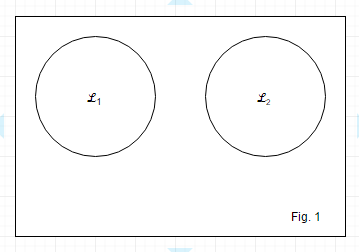
\includegraphics[width=1.0\textwidth]{parallel_fig1}\\
     Data dependency diagram of chosen decomposition
\end{figure}
\noindent Let $L$ be the set of numbers constructed from n such that $L = \{ L \in \mathbb{Z}\ |\ n \leq L \leq 1\}$.
Therefore let $L_1$ and $L_2$ be subsets of $L$ such that $L \in (L_1 + L_2) $.

\noindent Let $i \in \mathbb{Z} \ s.t. \ 0 \in i < n$.
Therefore $L_1 \in \{ n\ |\ (n - i)\ mod \ 2 = 0 \}$ and $L_2 \in \{ n\ |\ [(n - i) - 1]\ mod \ 2 = 0 \}$.\\\\


\begin{figure}
\centering
     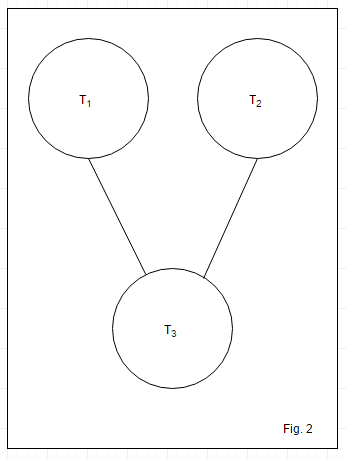
\includegraphics[scale=0.75]{parallel_fig2}\\
     Task interaction diagram of chosen decomposition
\end{figure}
\noindent Let $T_1$, $T_2$ and $T_3$ be the tasks which make up the decomposition of the factorial operation.\\
\\
\noindent $T_1$ uses the data-set $L_1$.\\
\noindent $T_2$ uses the data-set $L_2$.\\
\noindent $T_3$ uses the data-set $L_3$.\\
\\
\noindent $T_1$ and $T_2$ both iterate through their respective data-sets and multiply a running variable by the next number in their respective data-sets.
This variable is initialised by 1 and it becomes the answer of the previous iteration of the respective task. \\
\noindent $T_3$ is the task which multiplies the respective results of $T_1$ and $T_2$.\\\\


\begin{figure}
\centering
     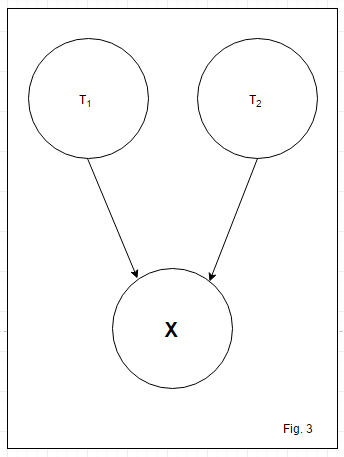
\includegraphics[scale=0.75]{parallel_fig3}\\
     Task dependency diagram of chosen decomposition
\end{figure}
\noindent $T_1$ and $T_2$ lead to a barrier, which is $T_3$. This operation waits for both $T_1$ and $T_2$ to complete and then a reduction operation occurs - denoted here by: $X$. $T_3$ takes the results of $T_1$ and $T_2$ and multiplies them together to get the final result, which means that both $T_1$ and $T_2$ have to complete before $T_3$ can be executed.\\\\


\section{Algorithm Complexity}
Assumptions made regarding the 
\noindent \chapter{Sequential Complexity:} \\
The complexity of the sequential algorithm is: $\ominus(n)$, where $n$ is the number being investigated as that many operations have to be completed to find the factorial.\\

\noindent \chapter{Recursive Complexity:} \\
The complexity of the recursive algorithm is: $\ominus(n + k)$, where $n$ is the number being investigated as that many operations have to be completed to find the factorial. $k$ is the arbitrary constant which represents the cost of the function recursively spawning itself $n$ times.\\

\noindent \chapter{Parallel Sequential Complexity:} \\
The time complexity of the decomposition of the sequential algorithm (The one from section 1) is: $\ominus(\frac{n}{2} + 1)$, where $n$ is the number being investigated as that many operations have to be completed to find the factorial and $1$ is the assumption that the reduction operator and final result takes constant time to complete. Another assumption that made is that both $T_1$ and $T_2$ complete their operations at roughly the same amount of time due to them having approximately the same number of operations to complete.\\

\noindent The computational complexity of this decomposition is: $\ominus(n + k)$, where $n$ is the number being investigated as that many operations have to be completed to find the factorial and $k$ is a constant that represents the complexity of the reduction operator and the complexity of the final operation. This is because the parallel version can complete its calculation faster than the standard iterative approach it cannot make the amount of computations required to complete the calculations any less.\\

\noindent \chapter{Parallel Recursive Complexity:} \\
The time complexity of a decomposition of the recursive algorithm is: $\ominus(\frac{n}{2} + k)$, where $n$ is the number being investigated and $k$ is a constant that represents the time taken due the reduction operations, wait factor of the different sections used and the time taken in memory due to executing the recursive operations of the algorithm.\\

\noindent The computational complexity of this decomposition is: $\ominus(n + k)$, where $n$ is the number being investigated as that many operations have to be completed to find the factorial and $k$ is a constant that represents the complexity of the reduction operator and the internal recursive nature of each section. This is because the parallel version can complete its calculation faster than the standard recursive approach it cannot make the amount of computations required to complete the calculations any less.\\ 

\section{OpenMP Implementation}


\end{page}
\end{document}
